\documentclass{article}
\usepackage[utf8]{inputenc}
\usepackage{indentfirst}
\usepackage{titling}
\usepackage{geometry}
\usepackage{graphicx}
\graphicspath{ {./Images/} }
\usepackage[shortlabels]{enumitem}
\usepackage{fancyhdr}
\usepackage{ulem}
\usepackage[dvipsnames]{xcolor}
\usepackage{amssymb}
\usepackage{listings}
\usepackage{color}

\definecolor{dkgreen}{rgb}{0,0.6,0}
\definecolor{gray}{rgb}{0.5,0.5,0.5}
\definecolor{mauve}{rgb}{0.58,0,0.82}

\lstset{frame=tb,
  language=Java,
  aboveskip=3mm,
  belowskip=3mm,
  showstringspaces=false,
  columns=flexible,
  basicstyle={\small\ttfamily},
  numbers=none,
  numberstyle=\tiny\color{gray},
  keywordstyle=\color{blue},
  commentstyle=\color{dkgreen},
  stringstyle=\color{mauve},
  breaklines=true,
  breakatwhitespace=true,
  tabsize=3
}

\def\ojoin{\setbox0=\hbox{$\bowtie$}%
  \rule[-.02ex]{.25em}{.4pt}\llap{\rule[\ht0]{.25em}{.4pt}}}
\def\leftouterjoin{\mathbin{\ojoin\mkern-5.8mu\bowtie}}
\def\rightouterjoin{\mathbin{\bowtie\mkern-5.8mu\ojoin}}
\def\fullouterjoin{\mathbin{\ojoin\mkern-5.8mu\bowtie\mkern-5.8mu\ojoin}}

\renewcommand\maketitlehooka{\null\mbox{}\vfill} %para centralizar verticalmente
\renewcommand\maketitlehookd{\vfill\null}
\pagestyle{fancy}
\fancyhf{}
\rfoot{\thepage}
\lfoot{ 
\includegraphics[scale=0.01]{UA.jpg} José Mendes 107188 LEI}
\geometry{
  a4paper,
  headheight=4cm,
  top=5.5cm,
  bottom=4.5cm,
  footskip=4cm
}


\title{Segurança Informática e nas Organizações}
\author{José Mendes 107188}
\date{2023/2024}

\begin{document}


\begin{titlepage}
    \maketitle
    \begin{center}
        
\includegraphics[scale=0.4]{UA.png}
    \end{center}
    \thispagestyle{empty} %remove o count da pagina
\end{titlepage}

\pagebreak

\section{Introdução}

\subsection{Segurança}

\begin{flushleft}
  \textbf{Segurança -} É o assunto focado na previsão de sistemas, processos, ambientes, \dots

  Ao longo de todos os aspetos do ciclo de vida de um sistema:
  \begin{itemize}
    \item Planeamento
    \item Desenvolvimento
    \item Execução
    \item Processos
    \item Pessoas
    \item Clientes e Supply Chain
    \item Mecanismos
    \item Standards e Regulamentos
    \item Propriedade Intelectual
  \end{itemize}
\end{flushleft}

\subsubsection{Planeamento}

Design de uma solução está de acordo com alguns requisitos dentro de um
contexto normativo.

\begin{flushleft}
  \textbf{Sem flaws}
  \begin{itemize}
    \item Todos os estados da operação são os previstos;
    \item Não há estados adicionais que fogem da lógica esperada (mesmo se transições forçadas são usadas);
  \end{itemize}

  \textbf{Dentro do scope de um contexto normativo}
  \begin{itemize}
    \item Especifico para cada atividade e setor (Ex: ISO 27001, ISO 27007, ISO 37001);
  \end{itemize}
\end{flushleft}

\subsubsection{Desenvolvimento}

Implementação de uma solução de acordo com o design, sem outros modos de operação.

\begin{flushleft}
  \textbf{Sem bugs a comprometer uma execução correta}
  \begin{itemize}
    \item Sem crashes;
    \item Sem resultados invalidos ou inesperados;
    \item Com tempos de execução corretos;
    \item Com consumo de recursos adequado;
    \item Sem leaks de informação;
  \end{itemize}

  \pagebreak

  \textbf{Software}
  \begin{itemize}
    \item Requer uma implementação cuidadosa;
    \item Requer testes para obter uma implementação com os comportamentos esperados;
  \end{itemize}
\end{flushleft}

\subsubsection{Execução}

Código executa tal como foi escrito, com todos os processos previstos.

\begin{flushleft}
  \textbf{O ambiente é controlado, não pode ser manipulado ou observado.}

  \textbf{Sem a existência de comportamentos anomalos, introduzido por aspetos ambientais} (como velocidade de armazenamento,
  quantidade de RAM, comunicação confiaveis)
\end{flushleft}

\begin{center}
  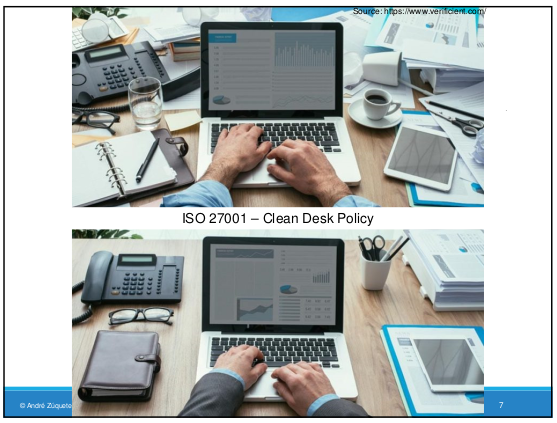
\includegraphics[scale=0.4]{1}
\end{center}

\subsubsection{Pessoas e Parceiros}

O comportamento do Staff não pode ter um impacto negativo na solução.

\begin{flushleft}
  \begin{itemize}
    \item As normas existem para regular que ações são expectáveis;
    \item O Staff é treinado para distinguir comportamento correto de comportamento incorreto;
    \item O Staff tem os incentivos corretos para se comportar adequadamente;
    \item Quando o Staff é comprometido, ou se desvia, as ações têm impacto limitado;
  \end{itemize}
\end{flushleft}

\pagebreak

\subsubsection{Análise e Audiroia}

Qual é o verdadeiro comportamento da solução?

\begin{flushleft}
  \textbf{Identificar desvios dos atributos experados}
  \begin{itemize}
    \item Faults, erros, comportamentos
  \end{itemize}

  \textbf{Identificar o risco para a solução ser modificada}
  \begin{itemize}
    \item Exposição a possíveis ataquantes;
    \item Incentivos que que alguém possa ter para modificar a solução;
    \item Identificar potenciais actors (threats);
  \end{itemize}

  \textbf{Identificar o impacto dos desvios}
  \begin{itemize}
    \item Perda total de dados? Denial of Service? Increase Operation Cost?
  \end{itemize}
\end{flushleft}

\begin{center}
  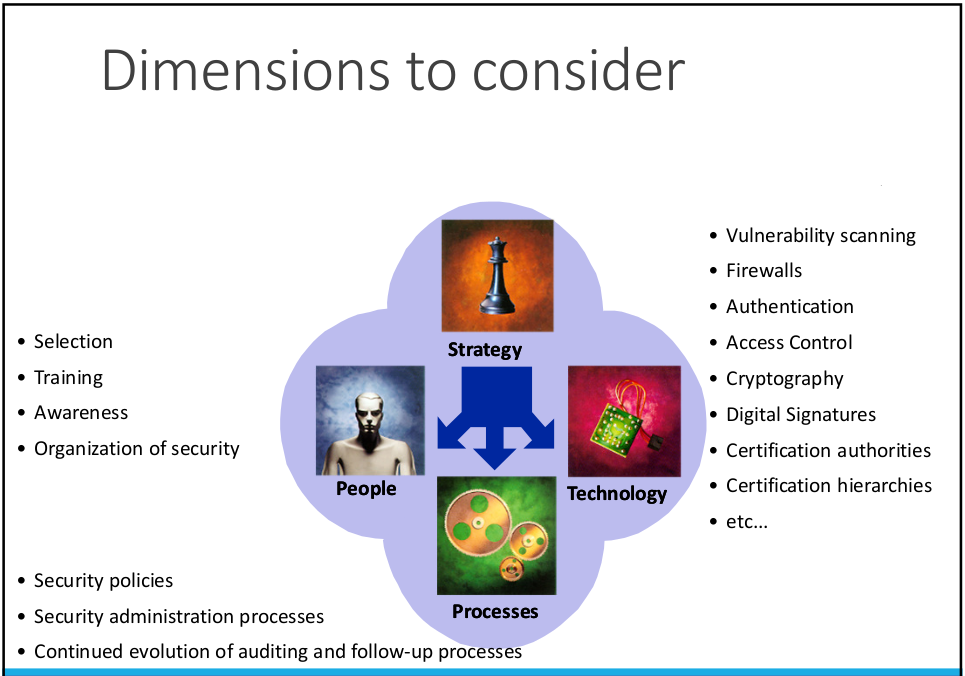
\includegraphics[scale=0.3]{2}
\end{center}

\subsection{Perspetivas}

A Segutrança tem muitas perspetivas interligadas.

\begin{flushleft}
  \textbf{Defensive:} Focado em manter previsão,

  \textbf{Offensive:} Focado em explorar a previsibilidade.
  \begin{itemize}
    \item Pode ter uma intenção maliciosa/criminosa;
    \item Pode ter como objetivo, a validação da solução (Red Teams);
  \end{itemize}

  \pagebreak

  \textbf{Outras:}
  \begin{itemize}
    \item Engenharia Inversa: Recuperar o design de porjetos contruidos;
    \item Forensics: Extrair informação e reconstruir eventos anteriores;
    \item Recuperação de Desastres: Minimizar o impacto de ataques;
    \item Auditoria: Avaliar se a solução está de acordo com um conjunto de requisitos;
  \end{itemize}
\end{flushleft}

\subsection{Objetivos de Segurança de Informação}

\begin{center}
  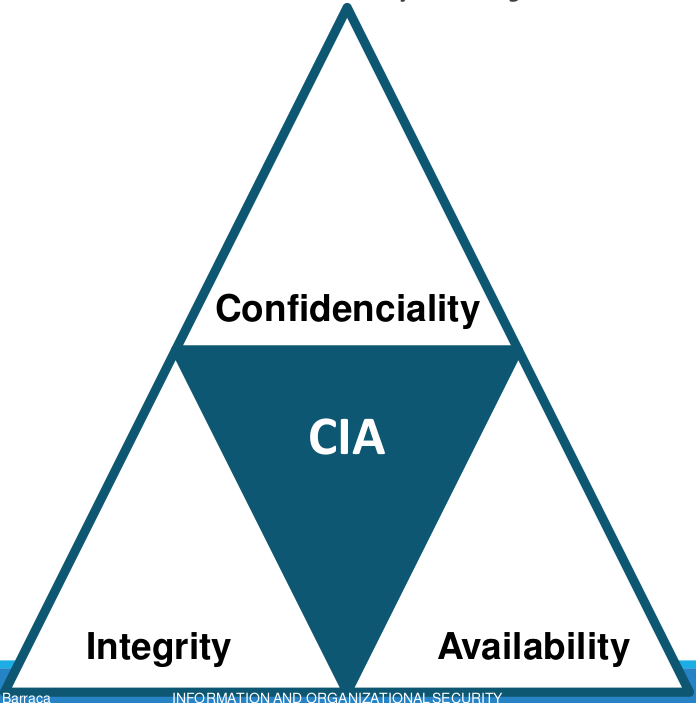
\includegraphics[scale=0.2]{3}
\end{center}

\begin{flushleft}
  \textbf{Confidencialidade:} A informação pode apenas ser acessada por um grupo restrito de entidades;
  
  \vspace{2mm}

  \uline{Medidas:}
  \begin{itemize}
    \item Encryptar informação;
    \item Usar passwords de acesso (fortes);
    \item Usar sistemas de gestão de identidade e autenticação;
    \item Doors, Strong Walls;
    \item Security personnel;
    \item Treinar (o Staff);
  \end{itemize}

  \vspace{2mm}

  \textbf{Integridade:} A informação permanece inalterada (Pode ser aplicada ao comportamento de dispositivos e serviços);

  \vspace{2mm}

  \uline{Medidas:}
  \begin{itemize}
    \item Controlo de identidade (hashes);
    \item Backups;
    \item Controlo de acesso;
    \item Dispositivos de armazenamento robustos;
    \item Processos de verificação de dados;
  \end{itemize}

  \pagebreak

  \textbf{Disponibilidade:} A informação está disponível a target entities (Pode ser aplicada aos serviços e dispositivos);

  \vspace{2mm}

  \uline{Medidas:}
  \begin{itemize}
    \item Backups;
    \item Planos de recuperação de desastres;
    \item Redundância;
    \item Virtualização;
    \item Monitorização;
  \end{itemize}

  \vspace{2mm}

  \textbf{Privacidade:} Como a informação pessoal é tratada (isto envolve:
  Obtida, Processada, Armazenada, Partilhada, Eliminada);

  \vspace{2mm}

  \uline{Medidas:}
  \begin{itemize}
    \item Controlo de acesso;
    \item Processos transparentes;
    \item Ciphers;
    \item Integridade e controlo de autenticação;
    \item Logs;
  \end{itemize}
\end{flushleft}

\subsection{Objetivos da Segurança}

\begin{flushleft}
  \textbf{Defesa contra eventos catastróficos:}
  \begin{itemize}
    \item Fenómenos naturais;
    \item Temperaturas extremas, inundações, trevoada, trovões, radiação, \dots
  \end{itemize}

  \textbf{Degradação do Hardware do computador:}
  \begin{itemize}
    \item Falha no fornecimento de energia;
    \item Bad sectors em discos;
    \item Bit errors em células RAM ou SSD;
  \end{itemize}

  \textbf{Defesa contra falhas normais:}
  \begin{itemize}
    \item Queda de energia;
    \item Falhas internas do sistema;
    \begin{itemize}
      \item Linux Kernel panic, Windows blue screen, OS X panic;
      \item Deadlocks;
      \item Uso anormal de recursos;
    \end{itemize}
    \item Falhas de software / Falhas de comunicação; 
  \end{itemize}

  \pagebreak

  \textbf{Defesa contra atividades não autorizadas (adversários):}
  \begin{itemize}
    \item Iniciado por alguém "de fora" ou "de dentro";
  \end{itemize}

  \uline{Tipos de atividades não autorizadas:}
  \begin{itemize}
    \item Acesso a informação;
    \item Alteração de informação;
    \item Utilização de recursos (CPU, memory, print, network, \dots);
    \item Denial of Service;
    \item Vandalismo (interferir com o funcionamento normal do sistema,
    sem obter benefícios);
  \end{itemize}
\end{flushleft}

\subsection{Conceitos Base}

\begin{enumerate}
  \item Domínios;
  \item Políticas;
  \item Mecanismos;
  \item Controlos;
\end{enumerate}

\subsubsection{Domínios}

Um conjunto de entidades que partilham atributos de segurança semelhantes.

\begin{flushleft}
  \begin{itemize}
    \item Permite gerir segurança de uma forma agregada;
    \begin{itemize}
      \item A gestão define os atributos do domínio;
      \item As entidades adicionadas ao domínio herdam os atributos do "grupo";
    \end{itemize}
    \item Comportamento e interações são homogéneas dentro do domínio;
    \item Domínios podem ser organizados em hierarquias;
    \item As interações entre domínios são, normalmente, controladas;
  \end{itemize}
\end{flushleft}

\begin{center}
  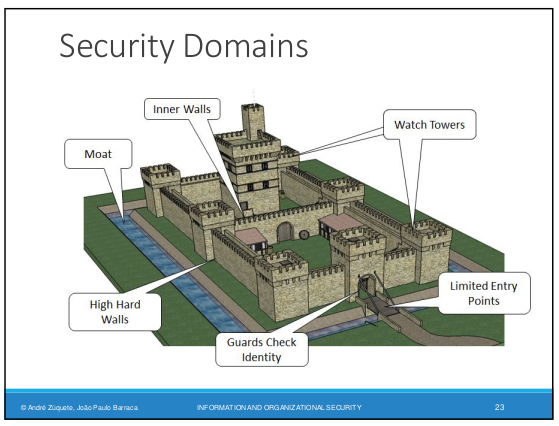
\includegraphics[scale=0.3]{4}
\end{center}

\pagebreak

\subsubsection{Políticas}

Conjunto de guidelnes relacionados com a segurança, que mandam sobre o domínio.

\begin{itemize}
  \item Organizações têm múltiplas políticas;
  \begin{itemize}
    \item Aplicavéis a cada domínio específico;
    \item Podem dar overlap e terem scopes diferentes/níveis abstratos;
  \end{itemize}
  \item As múltiplas políticas têm de ser coerentes;
  \item \uline{Exemplos:}
  \begin{itemize}
    \item Users apenas podem acessar serviços web;
    \item Os assuntos devem ser autenticados para entrar no domínio;
    \item Walls devem ser construidas de betão;
    \item Comunicações devem ser encriptadas;
  \end{itemize}
  \item Define o poder para cada assunto;
  \begin{itemize}
    \item Least privilege principle: cada assunto apenas deve ter os previlégios
    necessários para executar as suas tarefas;
  \end{itemize}
  \item Define procedimentos de segurança (quem faz o quê em que situação);
  \item Define os requisitos de segurança mínimos para um domínio;
  \begin{itemize}
    \item Security levels, Security Groups
    \item Autorização é necessária (and the related minimum authentication requirements (Strong/weak,
    single/multifactor, remote/face-to-face))
    \item Define estratégias de defesa e táticas de contra-ataque;
    \begin{itemize}
      \item Arquitetura defensiva;
      \item Monotorização de atividades criticas ou sinais de ataque;
      \item Reação contra ataques ou outros cenários anormais;
    \end{itemize}
    \item Define que atividades são legais e ilegais;
    \begin{itemize}
      \item Forbid list model: Some activities are denied, the rest are allowed;
      \item Permit list model: Some activities are allowed, the rest is forbidden;
    \end{itemize}
  \end{itemize}
\end{itemize}

\subsubsection{Mecanismos}

\begin{itemize}
  \item Implementam as políticas;
  \begin{itemize}
    \item Definem, num nível mais elevado, o que precisa de ser feito ou evitado;
    \item São usados para implementar políticas;
  \end{itemize}

  \pagebreak

  \item Mecânismos de segurnaça genéricos:
  \begin{itemize}
    \item Confinamento (sandboxing);
    \item Autenticação;
    \item Controlo de acesso;
    \item Execução priveligiada;
    \item Filtragem;
    \item Logging;
    \item Auditoria;
    \item Algoritmos criptográficos;
    \item Protocolos criptográficos;
  \end{itemize}
\end{itemize}

\begin{center}
  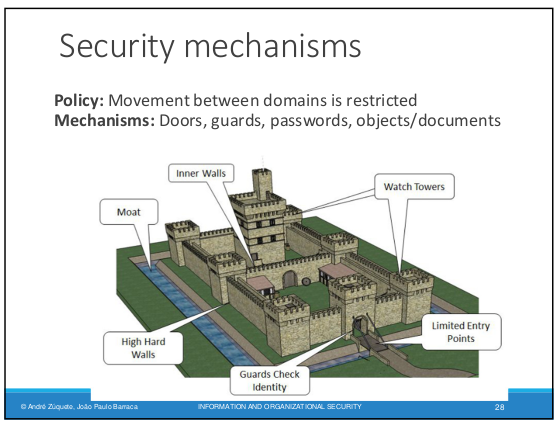
\includegraphics[scale=0.4]{5}
  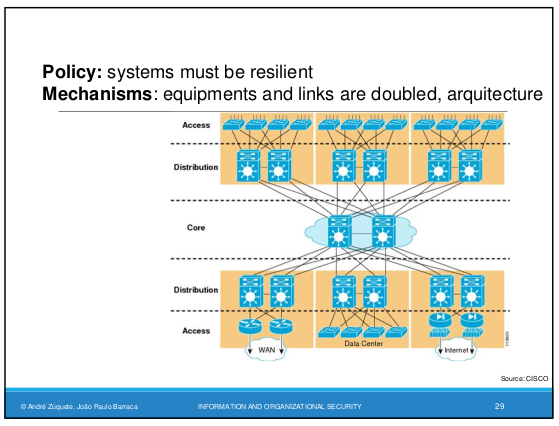
\includegraphics[scale=0.4]{6}
\end{center}

\pagebreak

\subsubsection{Controlos}

Controlos são quqlquer aspeto que permita minimizar o risco (proteger as propriedades \textbf{CIA})

\begin{flushleft}
  \begin{itemize}
    \item Controlos incluem políticas e mecanismos, mas também:
    \begin{itemize}
      \item Standards e regulamentos;
      \item Processos;
      \item Técnicas;
    \end{itemize}
    \item Controlos são explicitamente definidos e podem ser auditáveis;
    \begin{itemize}
      \item E.g.: ISO 27001 defines 114 controls in 14 groups (… asset management, physical security, incidente management…)
    \end{itemize}
  \end{itemize}
\end{flushleft}

\begin{center}
  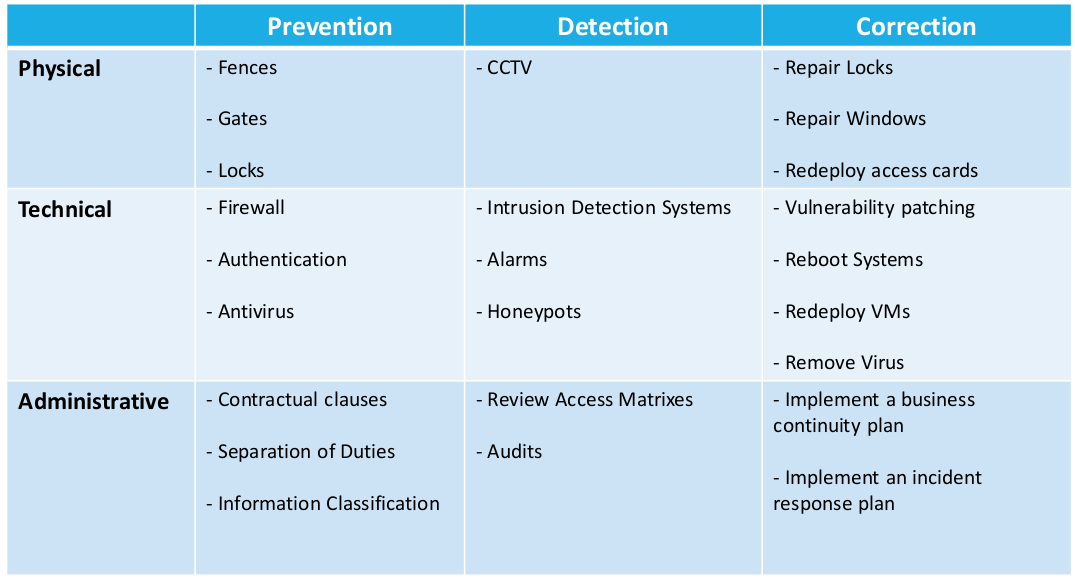
\includegraphics[scale=0.3]{7}

  Horizontal: Relação ao evento

  Vertical: Relação à sua natureza
\end{center}

\pagebreak

\subsection{Segurança na Prática}

Prevenção realista.

\begin{flushleft}
  \begin{itemize}
    \item \uline{Segurança perfeita é impossível};
    \item Focar nos eventos mais prováveis (pode depender de localização, legal framework, \dots)
    \item Considerar o custo e o profit;
    \begin{itemize}
      \item Um grande número de controlos tem um low cost;
      \item No entanto, não limite superior para o custo de uma estratégia de segurança;
    \end{itemize}
    \item Considerar todos os domínios e entidades;
    \begin{itemize}
      \item Um simples breach pode escalar para um problema maior;
    \end{itemize}
    \item Considerar impacto (Under the light of CIA and other potential impact areas (e.g., brand))
    \item Considerar o custo e o tempo de recuperação;
    \item Caracterizar ataquantes (definir controlos específicos para esses, vão
    sempre existir atacantes com mais recursos);
    \item Considerar que o sistema será comprometido (Ter planos de recuperação);
  \end{itemize}
\end{flushleft}

\subsection{Segurança em Sistemas Computacionais}

\begin{flushleft}
  \begin{itemize}
    \item Computadores podem fazer grandes danos em pouco tempo;
    \begin{itemize}
      \item Gerem grandes quantidades de informação;
      \item Processam e comunicam com grande velocidade;
    \end{itemize}
    \item O número de \textbf{weaknesses está sempre a aumentar};
    \begin{itemize}
      \item Devido a complexidade acrescida;
    \end{itemize}
    \item As redes permitem mecanismos de ataque mais sofisticados;
    \begin{itemize}
      \item Ataques anónimos de qualquer parte do mundo;
      \item Espalha-se rapidamente através de barreira geográficas;
      \item Exploitation of insecure hosts and applications
    \end{itemize}
    \item Os ataquantes constroem ataques em cadeia complexos;
    \begin{itemize}
      \item First exploration
      \item Lateral movement
      \item Exfilration
    \end{itemize}
  \end{itemize}

  \pagebreak

  \begin{center}
    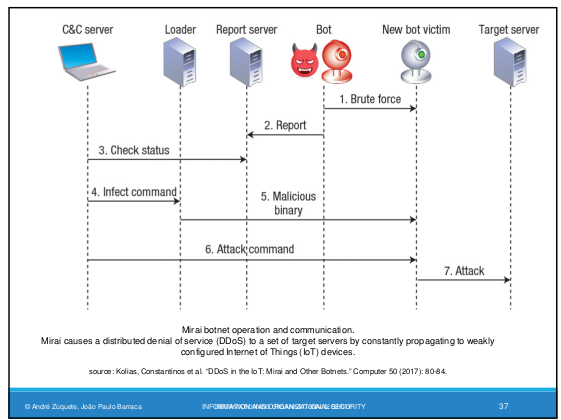
\includegraphics[scale=0.4]{8}
  \end{center}

  \begin{flushleft}
    \begin{itemize}
      \item A maior parte das vezes os users não sabem dos riscos
      \begin{itemize}
        \item Não sabem os problemas, impacto, boas práticas nem as soluções;
      \end{itemize}
      \item A maior parte das vezes os users são descuidados
      \begin{itemize}
        \item Porque tomam riscos;
        \item Não querem saber (não têm/identificam alguma responsabilidade);
        \item Não estimam o risco corretamente;
      \end{itemize}
    \end{itemize}
  \end{flushleft}

  \subsection{Maiores fontes de vulnerabilidades}

  \begin{flushleft}
    \textbf{Aplicações hostis ou com bugs}
    \begin{itemize}
      \item Rootkits: Insert elements in the operating system
      \item Worms: Software programs controlled by an attacker
      \item Virus: Pieces of code that infect other files (e.g., macros)
    \end{itemize}

    \textbf{Users}
    \begin{itemize}
      \item Ignorantes, descuidados, não querem saber
      \item Usam alternativas não seguras
      \item Confiam que as aplicações de segurança resolvem os problemas
      \item Download de software de fontes não confiáveis
      \item hostis
    \end{itemize}

    \textbf{Administração defeituosa}
    \begin{itemize}
      \item A configuração default é a mais segura
      \item Security restriction vs flexible operation
      \item Excessões a indivíduos
    \end{itemize}

    \pagebreak

    \textbf{Comunicação através de redes desconhecidas/não controladas}
    \begin{itemize}
      \item Public hotspots, campus networks, hostile governments
    \end{itemize}
  \end{flushleft}

  \subsection{Perimeter Defense}

  \begin{center}
    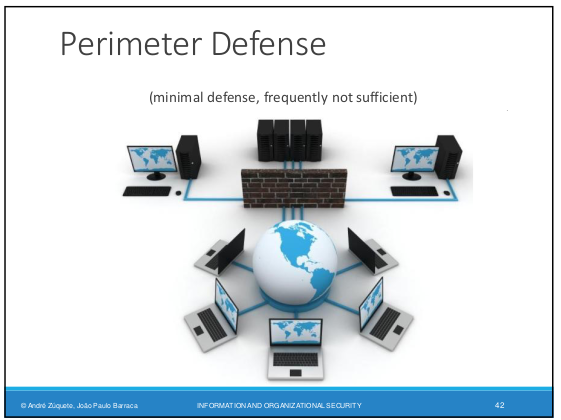
\includegraphics[scale=0.4]{9}
  \end{center}

  \begin{flushleft}
    \textbf{Proteção contra atacantes externos}
    \begin{itemize}
      \item Internet, Foreign users, outras organizações
    \end{itemize}

    \textbf{Assume que os users internos são confiáveis e partilham
    as mesmas políticas}
    \begin{itemize}
      \item Amigos, família, colaboradores
    \end{itemize}

    \textbf{Usados em cenários domésticos ou em pequenas empresas}

    \vspace{2mm}

    \textbf{Limitações:}
    \begin{itemize}
      \item Muito simples;
      \item Não protege contra ataques internos (users previamente confiáveis,
      atacantes que adquiriram acesso interno);
    \end{itemize}
  \end{flushleft}

  \subsection{Defesa em Profundidade}

  \begin{flushleft}
    \textbf{Proteção contra atacantes externos e internos}
    \begin{itemize}
      \item Da internet, de outras organizações, de users internos;
    \end{itemize}

    \textbf{Assume domínios bem definidos pela organização}
    \begin{itemize}
      \item Walls, doors, authentication, security personell, ciphers, secure networks
    \end{itemize}

    \textbf{Limitações}
    \begin{itemize}
      \item Precisa de coordenação entre os diferentes controlos (podemos acabar
      com controlos overlapping, mas também com "buracos" nos perímetros de segurança);
    \end{itemize}
  \end{flushleft}

  \pagebreak

  \subsection{Zero Trust}

  \begin{flushleft}
    \textbf{Modelos de defesa sem perímetros específicos}
    \begin{itemize}
      \item Não há confiança por herança nas entidades só por serem internas (
        na verdade, pode não haver noção de "interno" e "externo");
    \end{itemize}

    \textbf{Modelo recomendado para novos sistemas}
    \begin{itemize}
      \item Sistemas tradicionais deviam migrar para este modelo;
      \item Implies the design of systems/services specific for this model
      \item Legacy systems vão precisar de camadas de proteção adicionais (
        Firewalls, filtros, adapatadores, plugins)
    \end{itemize}
  \end{flushleft}

  \subsubsection{Princípios (NCSC)}

  \begin{enumerate}
    \item Saber a arquitetura (users, devices, services e data)
    \item Saber as identidades (users, devices, services e data)
    \item Avaliar o comportamento do user, service e saúde do device
    \item Usar políticas para autorizar requests
    \item Autenticar e autorizar em todo o lado (No open APIs, or IP address-based access)
    \item Focar a Monitorização nos users, devices e services
    \item Não confiar em nenhuma rede, incluindo a nossa (
      Os atacantes internos não devem ter mais privilégios que os externos)
    \item Escolher services feitos para \textbf{zero trust} (evitar legacy services, mas podem ser integrados)
  \end{enumerate}
  \end{flushleft}
  
  \pagebreak

  \section{Vulnerabilidades}

  \uline{Uma empresa é tão mais suscetível de ataques quanto maior a sua dimensão}, uma vez que
  ataques bem sucedidos serão mais rentáveis

  \vspace{2mm}

  De forma a prevenir \textbf{ataques}, que exploram \textbf{vulnerabilidades}, as organizações devem investir
  na \textbf{defesa} dos seus sistemas, de forma a garantir a segurança da informação que armazenam.

  \vspace{2mm}

  \subsection{Segurança de Informação}

  \begin{center}
    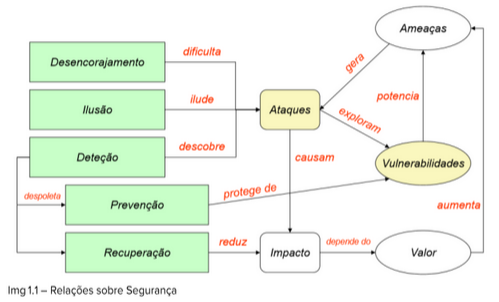
\includegraphics[scale=0.4]{10}
  \end{center}

  \subsubsection{Medidas (e algumas ferramentas)}

  No entanto, \textbf{defesa} é um conceito abstrato, que na realidade ganha forma em cinco medidas.

  \begin{flushleft}
    \textbf{Desencorajamento:} através da punição dos infratores (restrições legais e forensic evidences) e utilização de barreiras de segurança
    (firewalls, Autenticação, Sandboxing, \dots)

    \vspace{2mm}

    \textbf{Deteção:} sistema de deteção de intrusões (e.g Seek, Bro, Suricata), ou através de auditorias e análises forenses;

    \vspace{2mm}

    \textbf{Ilusão:} dos atacantes com honeypots ou honeynets (como que pishing para atacantes) e follow-up com análise forense;

    \vspace{2mm}

    \textbf{Prevenção:} através de políticas de segurança (e.g least priviledge principle), deteção (e.g OpensVas, metasploit) e correção de vulnerabilidades (e.g updates regulares);

    \vspace{2mm}

    \textbf{Recuperação:} com backups, sistemas redundantes, recuperação forense;
  \end{flushleft}

  \subsection{Vulnerabilidade}

  É um erro no software que pode ser diretamente usado por um atacante para
  ganhar acesso a um sistema ou rede.

  \begin{flushleft}
    Um erro é uma vulnerabilidade \uline{se permitir a um atacante usá-lo para violar
    uma política de segurança para esse sistema}.

    Isto exclui políticas de segurança completamente "abertas" em que todos os users
    são confiáveis, ou onde não há consideração do risco do sistema.

    \pagebreak

    Uma vulnerabilidade \textbf{CVE} é um estado num sistema computacionas
    (ou conjunto de sistemas) que podem:
    \begin{itemize}
      \item Permitir ao atacante executar comandos como outro user;
      \item Permitir ao atacante aceder a dados que é contrário às restrições
      de acesso específicadas para esses dados;
      \item Permitir a um atacante fingir ser outra entidade;
      \item Permitir ao atacante realizar denial of service;
    \end{itemize}
  \end{flushleft}

  \subsection{Exposição}

  Problema de \uline{configuração} que permite ao atacante aceder a informação ou capacidades que o podem
  auxiliar, sem conseguir no entanto comprometer diretamente o sistema.

  \vspace{2mm}

  \textbf{Um problema de configuração ou um erro é uma exposição se não permitir
  diretamente comprometer a segurança do sistema}, mas pode ser um componente
  importante para a realização de um ataque bem sucedido, e é uma violação
  de uma política de segurança.

  \vspace{2mm}

  \textbf{Uma exposição descreve um estado no sistema computacional (ou conjunto de sistemas)
  que não é uma vulnerabilidade mas pode:}
  \begin{itemize}
    \item Permitir a um atacante conduzir atividades para obter informação;
    \item Permitir a um atacante esconder atividades;
    \item Inclui uma capacidade que se comporta como esperado, mas pode ser
    facilmente abusada;
    \item É o ponto primário de entrada em que um atacante pode tentar
    usar para ganhar acesso ao sistema ou aos dados;
    \item É considerado um poblema por algumas políticas de segurança;
  \end{itemize}

  \subsection{CVE - Common Vulnerabilities and Exposures}

  É um repositório público de vulnerabilidades, que lista e descreve vulnerabilidades e
  exposições de segurança.

  \vspace{2mm}

  \textbf{Dicionário de vulnerabilidades e exposições sobre segurança de informação}
  \begin{itemize}
    \item Para gestão de vulnerabilidades;
    \item Para gestão de resolução de problemas;
    \item Para alertar sobre novas vulnerabilidades;
    \item Para deteção de intrusões;
  \end{itemize}

  \pagebreak

  \textbf{Usa identificadores comuns para os mesmos CVEs}
  \begin{itemize}
    \item Permite a partilha de dados entre produtos de segurança;
    \item Oferece um baseline index point para avaliar coverage of
    tools and services;
  \end{itemize}

  \textbf{Detalhes sobre uma vulnerabilidade podem ser mantidos privados}
  \begin{itemize}
    \item Parte da divulgação responsável: até que o proprietário forneça uma solução;
  \end{itemize}

  \vspace{2mm}

  (Ver imagem no slide 4)

  \subsubsection{Identificadoes CVE}

  \textbf{Aka CVE names, CVE numbers, CVE-IDs, CVEs}

  \vspace{2mm}

  \textbf{Identificador único e comum para vulnerabilidades de segurança de informação publicamente conhecidas}
  \begin{itemize}
    \item Têm status "candidate" ou "entry";
    \item Candiddato: Em review para inclusão na lista;
    \item Entry: Aceite na lista CVE;
  \end{itemize}

  \vspace{2mm}

  \textbf{Formato}
  \begin{itemize}
    \item Numero identificador CVE (CVE-Year-Order);
    \item Status (candidate, entry);
    \item Descrição curta da vulnerabilidade ou exposição;
    \item Referências a fontes de informação;
  \end{itemize}

  \subsubsection{Benefícios do CVE}

  \textbf{Fornece uma linguagem comum para os problemas referenciados}
  \begin{itemize}
    \item Facilita a partilha de dados entre ferramentas e serviços;
    \item Sistemas de deteção de intrusões;
    \item Ferramentas de acesso;
    \item Bases de dados de vulnerabilidades;
    \item Researchers;
    \item Equipes de resposta a incidentes;
  \end{itemize}

  \vspace{2mm}

  \textbf{Vai liderar para melhorar as ferramentas de segurança} (mais compreensívo,
  melhores comparações, interoperabilidade)

  \vspace{2mm}

  \textbf{Vai originar mais inovação} (Ponto focal para discutir questões críticas de conteúdo de banco de dados)

  \subsubsection{CVE e ataques}

  Ataques são tornados possíveis através de múltiplas vulnerabilidades (um CVE para cada vulnerabilidade)

  

  \subsection{Deteção de Vulnerabilidades}

  \textbf{Ferramentas específicas podem ser usadas para detetar vulnerabilidades}

  Estas exploram vulnerabilidades conhecidas, testando padrões (e.g buffer overflow, SQL injection, XSS, \dots)

  \vspace{2mm}

  \textbf{Ferramentas específicas podem replicar ataques conhecidos}

  Usar exploits conhecidos para vulnerabilidades conhecidas. Podem ser usadas
  para implementar medidas de defesa.

  \vspace{2mm}
  
  \textbf{Vital para certificar a robustez de um sistema de produção e aplicações}

  Serviço muitas vezes oferecido por empresas externas.

  \vspace{2mm}

  \textbf{Pode ser aplicado a:}
  \begin{itemize}
    \item Source code;
    \item Aplicações em execução (análise dinâmica);
    \item Externamente como um cliente remoto;
  \end{itemize}

  \vspace{2mm}

  \textbf{Não dever ser aplicado \uline{cegamente} a sistemas de produção}

  Potencial perda de dados/corrupção, DoS, atividade ilegal, \dots

  \subsection{CWE - Common Weakness Enumeration}

  De forma complementar temos outro repositório, mas focado na exploração das causas das
  vulnerabilidades, ou seja, identifica as vulnerabilidades provocadas pelos
  developers devido a
  uma utilização incorreta do
  software.

  \vspace{2mm}

  São encontradas no código, design, arquitetura do sistema. Cada CWE representa
  um único tipo de vulnerabilidade. É mantido pelo MITRE e esta lista
  fornece detalhes para cada CWE.
  
  \vspace{2mm}

  Um CWE podem organizar-se de forma hierárquica, havendo um pai que fornece uma descrição genérica e vários
filhos, cada um focado numa parte concreta do problema.

\vspace{2mm}

  Níveis mais profundos de CWEs, oferecem mais granularidade, normalmente
  com menos filhos, ou sem filhos.

  \begin{center}
    \subsubsection*{CWE $\ne$ CVE}
  \end{center}

  \pagebreak

  \begin{center}
    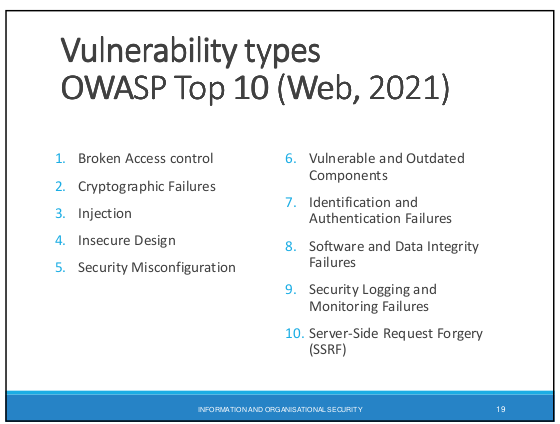
\includegraphics[scale=0.35]{11}
    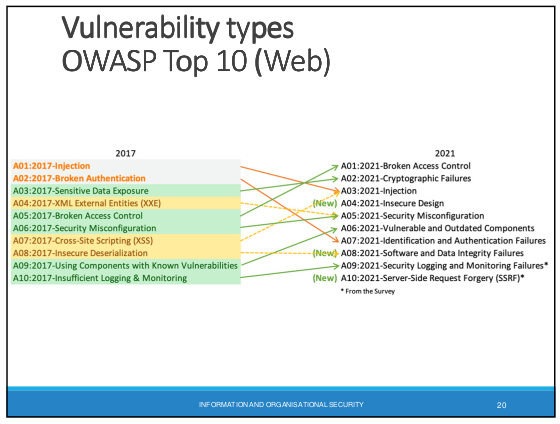
\includegraphics[scale=0.35]{12}
  \end{center}

  \subsection{Rastreamento de Vulnerabilidades por parte dos vendedores}

  Durante o ciclo de desenvolvimento, as vulnerabilidades são tratadas como bugs,
  pode existir uma equipa de segurança ou não. Qunado o software está disponivel,
  as vulnerabilidades também sõa rastreadas globalmente, para cada sistema
  e software disponivel ao público.

  \vspace{2mm}

  O rastreamento público ajuda a:
  \begin{itemize}
    \item Focar a discussão à volta do problema;
    \item Aos defensores a facilmente testar o sistema, aumentando a segurança;
    \item Aos atacantes a facilmente saberem quais as vulnerabilidades a explorar;
  \end{itemize}

  \vspace{2mm}

  As vulnerabilidades são rastreadas de forma privada (consitui um arsenal para
  ataques futuros contra alvos)

  \vspace{2mm}

  O conhecimento sobre vulnerabilidades é publicamente disponível e pode
  ser trocado por dinheiro. Mas também pode ser trocado de forma privada
  por ainda mais dinheiro.


  \subsection{Rastreamento de Vulnerabilidades}

  Não é algo fácil de fazer, uma ver que os exploits não são sempre
  conhecidos, o impacto e o custo podem ser difíceis de estimar (underestimated).

  \vspace{2mm}

  Feeds anteriores podem criar um falso sentido de segurança.

  \vspace{2mm}

  Possuir uma \textbf{comunicação dinâmica} é bom:
  \begin{itemize}
    \item \uline{Para os defensores}, pois eles podem testar e implementar defesas;
    \item \uline{Para atacantes}, pois estes podeqm incorporar os exploits;
  \end{itemize}

  \pagebreak

  \subsection{Ataques de dia zero}

  Aka Zero Day (or Zero Hour) Attacks/Threat.

  \vspace{2mm}

  Este tipo de ataque caracteriza-se por \uline{explorar uma vulnerabilidade desconhecida}.
  Este ocorre no dia zero do conhecimento da vulnerabilidade, para a qual não existe
  um security fix.

  \vspace{2mm}

  Se for explorada de forma discreta, pode durar meses ou até anos, conhecido
  por atacantes e não pelos outros, frequentemente parte do arsenal de ataque, sendo inclusive
  comercializadas em certos mercados (negro).

  \subsection{Sobrevivência}

  Como sobreviver a um ataque Dia Zero? Como podemos reagir a um destes ataques?

  \vspace{2mm}

  Apesar de ser o oposto do que geralmente é esperado dos sistemas (estandardização,
protocolos bem definidos e regulares), a \textbf{diversidade} é a chave para a sobrevivência.

\vspace{2mm}

Isto porque dada a sua exclusividade, operações e protocolos distintos são mais difíceis de
contornar, uma vez que requerem um estudo dedicado do sistema em particular e não podem
ser aplicados de forma generalizada a outros.

\vspace{2mm}

Dada a sua diversidade, o SO Android terá menos probabilidade de ser atacado que o iOS.

\subsection{CERT - Computer Emergency Readiness Team}

Esta é uma \uline{equipa responsável por resistir a ataques} em sistemas distribuídos (em rede),
limitando o dano e garantindo a continuidade dos serviços críticos.

\vspace{2mm}

\subsubsection*{CERT/CC (Coordination Center) @ CMU}

Um componente de um maior programa CERT, é um centro importante
para problemas de segurança na internet.

\subsection{CSIRT - Computer Security Incident Response Team}

Dentro das equipas CERT, há uma componente de sigla CSIRT, cuja responsabilidade é
receber, analisar e responder a relatórios de incidente e atividade.

\subsection{Alertas de Segurança e activity trends}

Vital para a disseminação rápida de conhecimento sobre novas vulnerabilidades
(e.g US-CERT Cyber Security Alerts, SANS Internet Storm Center, Cisco Security Center, \dots)

\pagebreak

\section{Modelos de Controlo de Acesso}

\subsection{Tipos de Acesso}

\begin{flushleft}
  \textbf{Acesso Físico:} Contacto físico entre o sujeito e o objeto de interesse
  (e.g. acesso a um edifício, internet, computador, aparelho, tocken \dots)

  \textbf{Acesso Informático ou Eletrónico:} Contacto orientado à informação entre
  o sujeito e o objeto de interesse, isto é, contacto através de dialogos
  request-response. Este contacto é mediado por computadores, redes,
  sistemas operativos, aplicações, middleware, \dots
\end{flushleft}

\subsection{Controlo de Acesso}

\begin{center}
  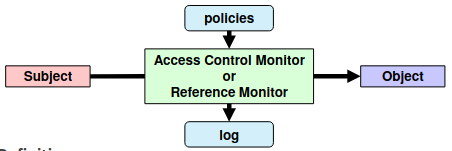
\includegraphics[scale=0.4]{13}
\end{center}

Políticas e mecânismos que mediam o acesso do sujeito a um objeto.

\vspace{2mm}

\begin{flushleft}
  \textbf{Requisitos Normais (AAA):}
  \begin{itemize}
    \item Autenticação (com algum Level of Assurange (LoA))
    \item Políticas de Autorização
    \item Acountability (Auditoria) $\rightarrow$ logging
  \end{itemize}
\end{flushleft}

Sujeitos e objetos são os dois \uline{entidades digitais}.

\begin{flushleft}
  \textbf{Sujeitos:} Algo exibindo atividade (e.g. processos, computadores, redes)

  \vspace{2mm}

  \textbf{Objetos:} O alvo da ação (e.g. dados armazenados, tempo de CPU,
  memória, processos, computadores, redes)

  \vspace{2mm}

  \textbf{Nota:} Uma entidade pode ser um sujeito e um objeto ao mesmo tempo.
\end{flushleft}

\subsection{Princípio do Menor Privilégio aka Least Privilege Principle}

Todos os programas e todos os utilizadores do sistema devem operar usando
o menor conjunto de privilégios necessários para completar o trabalho.

\vspace{2mm}

\begin{flushleft}
  \textbf{Privilégios:} Autorização para executar um dado trabalho, parecido
  com access control clearance.
\end{flushleft}

Cada sujeito deve ter, em todo o momento, o número de privilégios exato necessário
para completar os trabalhos dados. Menos previlégios criam
barreiras intrespassáveis, enquanto que mais privilégios criam Vulnerabilidades
(dano causado por acidentes ou erros, má utilização de privilégios, \dots)

\pagebreak

\subsection{Modelos de Controlo de Acesso}

\begin{center}
  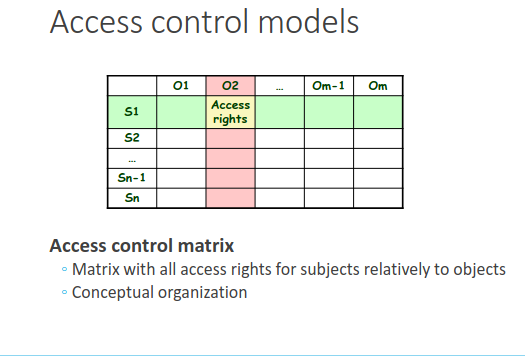
\includegraphics[scale=0.4]{14}
\end{center}

\begin{flushleft}
  \textbf{Mecânismos ACL-based:} ACL: Access Control List, coluna da matrix

  \vspace{2mm}

  \textbf{Lista de direitos de acesso para sujeitos especificos:} Os direitos de
  acesso podem ser positivos e negativos, sujeitos base podem ser usados normalmente.
  
  \vspace{2mm}

  \textbf{Normalmente, ACLs estão guardados com os objetos}

  \vspace{2mm}

  \textbf{Mecânismos Capability-based:} Capability: token de autorização impossivel
  de falsificar, linha da matrix, contém referências a objetos e direitos de acesso.

  \vspace{2mm}

  \textbf{Conceder acesso:} Transmissão de capabilities entre sujeitos (mediado/não mediado)

  \vspace{2mm}

  \textbf{Normalmente, capabilities estão guardados com os sujeitos}
\end{flushleft}

\subsubsection{Tipos de Controlo de Acesso: MAC e DAC}

\begin{flushleft}
  \textbf{Mandatory Access Control (MAC):}
  \begin{itemize}
    \item Política de controlo de acesso é fixa e implementada
    pelo monitor de controlo de acesso;
    \item Os direitos de controlo de acesso não podem ser adaptados
    pelos sujeitos ou pelos donos dos objetos;
  \end{itemize}

  \vspace{2mm}

  \textbf{Discretionary Access Control (DAC):}
  \begin{itemize}
    \item Alguns sujeitos podem alterar os direitos dados ou negados
    a outros sujeitos para um dado objeto;
    \item Normalmente, isto é dado aos donos dos objetos e aos
    administradores do sistema;
  \end{itemize}
\end{flushleft}

\subsubsection{Tipos de Controlo de Acesso: Role-Based Access Control (RBAC)}

\begin{flushleft}
  \textbf{Não é nem MAC nem DAC}
  \begin{itemize}
    \item Os roles são dinamicamente atribuidos aos sujeitos;
    \item Para controlo de acesso, o role importa usado pelo sujeito
    e não a identidade do sujeito (a identidade é mais relevante para acesso
    a roles e logging);
  \end{itemize}

  \pagebreak

  \textbf{Controlo de Acesso vincula funções a operações (significativas)}
  \begin{itemize}
    \item Operações são transações de sistema complexas e significativas;
    \item Operações podem envolver múltiplos objetos individuais lower-level;
  \end{itemize}
\end{flushleft}

\subsubsection{Regras RBAC}

\begin{flushleft}
  \textbf{Atribuição de roles:}
  \begin{itemize}
    \item Toda a atividade do sujeito num sistema é conduzida através de transações.
    As transações são permitidas para roles específicos, logo, todos os sujeitos têm de ter
    algum role ativo;
    \item Um sujeito pode executar uma transação \textbf{apenas se} tiver selecionado/tiver
    sido atribuido o role que permite a execução dessa transação;
  \end{itemize}

  \vspace{2mm}

  \textbf{Autorização de role:} O role ativo de um sujeito tem de ser autorizado para esse sujeito;

  \vspace{2mm}

  \textbf{Autorização de transação:} Um sujeito pode executar uma transação \textbf{apenas se}
  essa transação for autorizada através dos role membership's do sujeito e
  se não houver nenhuma limitação que possa ser aplicada sobre sujeitos, roles e permissões. 
\end{flushleft}

\begin{center}
  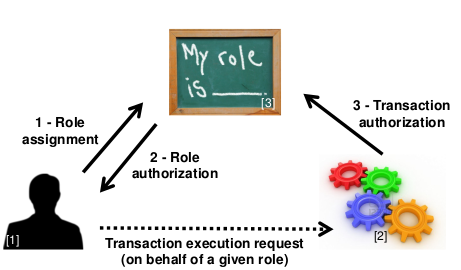
\includegraphics[scale=0.4]{15}
\end{center}

\subsubsection{RBAC: Roles e Groups}

\begin{flushleft}
  \textbf{Roles:} São uma coleção de permissões que são atribuidas aos sujeitos, que num
  determinado instante têm esse role. Um sujeito pode (deve) apenas ter um role ativo de cada vez.

  \vspace{2mm}

  \textbf{Groups:} São conjuntos de users, e as permissões podem ser atribuidas
  a ambos, users e groups. Um sujeito pode pertemcer a vários grupos ao mesmo tempo.

  \vspace{2mm}

  \textbf{O conceito de sessão:} A atribuição de um role é tipo a ativação de uma sessão.
  O group membership é um atributo estático ordinário.
\end{flushleft}

\begin{center}
  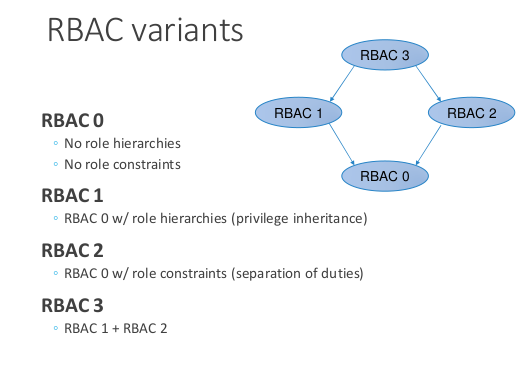
\includegraphics[scale=0.4]{16}
\end{center}

\subsubsection{Modelo NIST RBAC}

\begin{flushleft}
  \textbf{Flat RBAC:} Simples modelo RBAC, com \textbf{user-role review}
  \begin{center}
    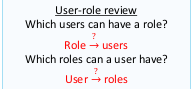
\includegraphics[scale=0.6]{17}
  \end{center}

  \vspace{2mm}

  \textbf{Hierarchical RBAC:} Flat RBAC com \textbf{role hierarchies} (DAG ou árvore).
  Hierarquias gerais e restritas.

  \vspace{2mm}

  \textbf{Constrained RBAC:} RBAC com \textbf{role constraints} para separar
  deveres.

  \vspace{2mm}

  \textbf{Symmetric RBAC:} RBAC com \textbf{permission-role review}
  \begin{center}
    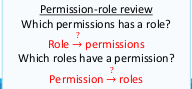
\includegraphics[scale=0.6]{18}
  \end{center}
\end{flushleft}

\subsubsection{Tipos de Controlo de Acesso: Context-Based Access Control (CBAC)}

\begin{flushleft}
  \textbf{Os direitos de acesso têm um contexto histórico}, não podem ser
  determinados sem considerar operações de acesso anteriores.

  \vspace{2mm}

  \textbf{Chinese Wall Policy:} Grupos conflituantes, políticas de controo de acesso
  devem considerar acessos passados a objetos em diferentes membros de grupos conflituantes.
\end{flushleft}

\subsubsection{Tipos de Controlo de Acesso: Attribute-Based Access Control (ABAC)}

\begin{flushleft}
  \textbf{Decisões de controlo de acesso são baseadas em atributos associados
  a entidades relevantes}

  \pagebreak

  \textbf{Arquitetura OASIS XACML:}
  \begin{itemize}
    \item Policy Administration Point (PAP), onde as políticas são geridas
    \item Policy Decision Point (PDP), onde as decisões de autorização são avaliadas e tomadas
    \item Policy Enforcement Point (PEP), onde os pedidos de acesso são intercetados e
    confrontados com decisões PDP
    \item Policy Information Point (PIP), onde o PDP obtém informação externa
  \end{itemize}
\end{flushleft}

\subsubsection{XACML: Controlo de Acesso com PEP e PDP}

\begin{flushleft}
  \textbf{Um sujeito realiza um pedido}, intercetado pelo PEP, que envia o pedido
  de autorização para o PDP.

  \vspace{2mm}

  \textbf{O PDP avalia o pedido contra as suas políticas e chega a uma decisão},
  que é returnada pelo PEP.
  
  \begin{itemize}
    \item As políticas são devolvidas por um Policy Retrieval Point (PRP)
    \item Atributos úteis são obtidos por um Policy Information Point (PIP)
    \item As políticas são geridas pelo Policy Administration Point (PAP)
  \end{itemize}
\end{flushleft}

\begin{center}
  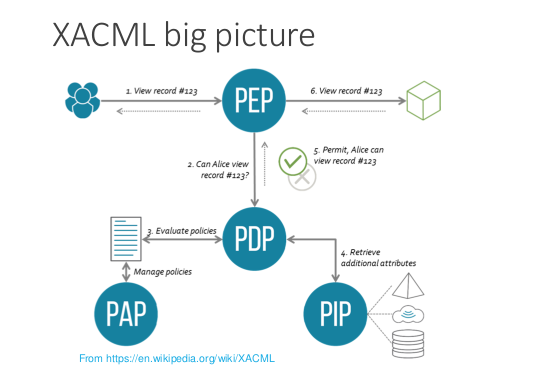
\includegraphics[scale=0.4]{19}
\end{center}

\subsection{Modelos de Controlo de Acesso: Break-the-Glass}

\begin{flushleft}
  \textbf{Em alguns cenários, pode ser necessário utrpassar os limites de acesso estabelecidos}
  (e.g questão de vida ou morte).

  \vspace{2mm}

  \textbf{Neste casos, o sujeito pode usar uma decisão break-the-glass sobre a recusa de acesso}.
  Ultrapassa a recusa com a própria responsabilidade, logging é fundamental para
  prevenir abusos.
\end{flushleft}

\pagebreak

\subsection{Separação de Deveres}

\begin{flushleft}
  \textbf{Requisito fundamental de segurança para prevenção de fraude e erro}.
  Disseminação de tarefas e privilégios associados, para um negócio específico,
  por múltiplos sujeitos. Muitas vezes implementado com RBAC.
  
  \vspace{2mm}

  \textbf{Controlo de Danos}. Segregação de deveres ajuda a reduzir os potenciais
  danos das ações de uma pessoa. Alguns deveres não devem ser combinados numa única posição.
\end{flushleft}

\subsection{Modelos do flow de informação}

\begin{flushleft}
  \textbf{Autorizaçao é aplicada ao flow dos dados}
  \begin{center}
    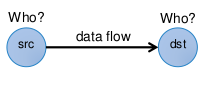
\includegraphics[scale=0.4]{20}
  \end{center}
  Objetivo: envitar flows de informação que não queremos/perigosos

  \vspace{2mm}

  \textbf{Atributos de segurança Src e Dst}, o flow apenas deve acontecer entre duas entidades
  com os atributos de segurança apropriados. A autorização é baseada nos atributos de segurança (SL).
\end{flushleft}


\subsection{Segurança Multinível}

\begin{flushleft}
  \textbf{Sujeitos (ou roles) atuam em diferentes níveis de segurança}. Este níveis não
  se intersetão a si próprios, e possuem uma ordem parcial (hieraruquia, lattice).
  \begin{center}
    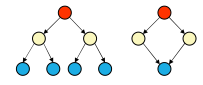
\includegraphics[scale=0.4]{21}
  \end{center}

  \vspace{2mm}

  \textbf{Os níveis são usados como atributos dos sujeito e dos objetos}.
  \begin{itemize}
    \item \textbf{Sujeitos:} clearance a nível de segurança;
    \item \textbf{Objetos:} classification a nível de segurança;
  \end{itemize}

  \vspace{2mm}

  \textbf{Flows de informação e níveis de segurança}
  \begin{itemize}
    \item Mesmo nível de segurança: atutorizado;
    \item Nível de segurança diferente: controlado;
  \end{itemize}

  \pagebreak

  \begin{center}
    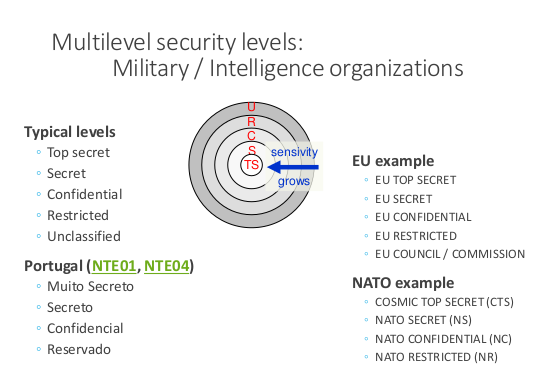
\includegraphics[scale=0.4]{22}
  \end{center}
\end{flushleft}

\subsection{Categorias de segurança (ou compartimentos)}

\begin{flushleft}
  \textbf{Ambientes de self-contained information}, podem abrager
  vários níveis de segurança.

  \vspace{2mm}

  \textbf{Ambientes militar}, ramos militares, unidades militares

  \vspace{2mm}

  \textbf{Ambientes civís}, departamentos, unidades de organização

  \vspace{2mm}

  \textbf{Um objeto pode pertencer a diferentes compartimentos e
  ter diferentes classificações de segurança para cada um} ((top-secret, crypto),
  (secret, weapon))

  \begin{center}
    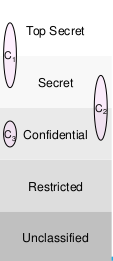
\includegraphics[scale=0.4]{23}
  \end{center}
\end{flushleft}

\subsection{Labels de segurança}

\begin{center}
  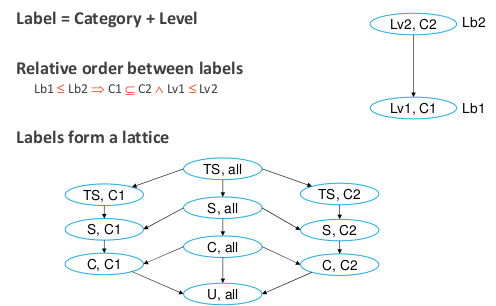
\includegraphics[scale=0.4]{24}
\end{center}

\pagebreak

\subsection{Modelos MLS Bell-La Padula}

\begin{flushleft}
  \textbf{Política de controlo de acesso para controlar flows de informação}.
  Aborda a confidencialidade dos dados e o acesso a informação classificada. Aborda
  a divulgação de informação classificada (controlo de acesso dos objetos não é suficiente).

  \vspace{2mm}

  \textbf{Usa um modelo de transação de estados}. Em cada estado há sujeitos, objetos,
  uma matrix de acesso e a informação atual de acesso. Regras de transação de estados.
\end{flushleft}
\begin{center}
  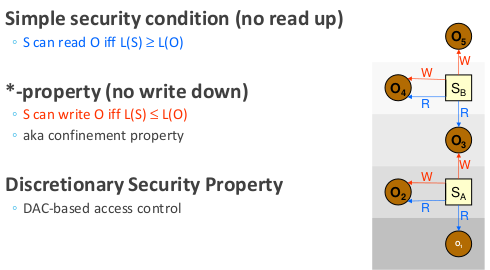
\includegraphics[scale=0.4]{25}
\end{center}

\subsection{Modelo de Integridade Biba}

\begin{flushleft}
  \textbf{Política de controlo de acesso para controlar flows de informação}.
  \begin{itemize}
    \item Para reforçar o controlo da integridade dos dados;
    \item Usa níveis de integridade, não níveis de segurança;
    \item Parecido com \textbf{Bell-La Padula} com regras invertidas;
  \end{itemize}

  \begin{center}
    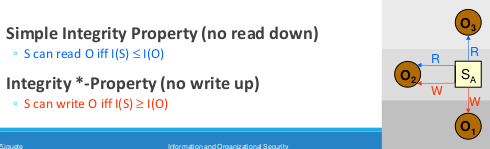
\includegraphics[scale=0.4]{26}
  \end{center}
\end{flushleft}

\subsection{Controlo de Integridade obrigatório Windows}

\begin{flushleft}
  \textbf{Permite controlo de acesso obrigatório antes de avaliar DACLs}
  \begin{itemize}
    \item Se não for permitido, DACLs não são avaliadas;
    \item Se for permitido, DACLs são avaliadas;
  \end{itemize}

  \pagebreak

  \textbf{Labels de integridade}
  \begin{itemize}
    \item Não confiável;
    \item Baixo (ou AppContainer);
    \item Médio;
    \item Médio Plus;
    \item Alto;
    \item Sistema;
    \item Processo Protegido;
  \end{itemize}

  \vspace{2mm}

  \textbf{Users}
  \begin{itemize}
    \item \uline{Médios}: users normais;
    \item \uline{Altos}: users elevados;
  \end{itemize}

  \vspace{2mm}

  \textbf{Processos de nível de integridade}
  \begin{itemize}
    \item O minímo associado ao owner e ao ficheiro executável;
    \item Processos de um user normalmente são \textbf{médio} ou \textbf{alto} (exceto
    ao executar ficheiros executáveis \textbf{Low}-labeled);
    \item Processos de serviço: \textbf{alto};
  \end{itemize}
\end{flushleft}

\begin{center}
  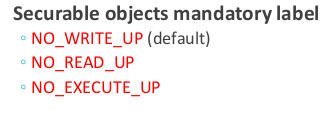
\includegraphics[scale=0.4]{27}
\end{center}

\pagebreak

\section{Sistemas Operativos}

\begin{center}
  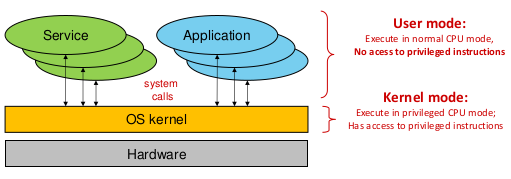
\includegraphics[scale=0.4]{28}
\end{center}

\subsection{Objetivos do Kernel}

\begin{flushleft}
  \begin{itemize}
    \item Inicia os dispositivos (boot time);
    \item Virtualiza o hardware, modelo computacional;
    \item Reforça políticas de proteção e fornece mecânismos de proteção. Contra
    erros involuntários e atividades não autorizadas;
    \item Fornece o sistema de ficheiros, independente dos dispositivos de armazenamento usados;
  \end{itemize}
\end{flushleft}

\subsection{Anéis de Execução}

\begin{flushleft}
  \textbf{Diferentes níveis de privilégio}, formando um conjunto de anéis. Usado
  pelos CPUs para prevenir código não priveligiado de correr opcodes privilegiados.

  \vspace{2mm}

  \textbf{Hoje em dia, os processadores têm 4 anéis}, mas apenas 2 são usados pelo OS,
  o 0 e o 3. O 0 é o mais privilegiado (supervisor/kernel mode) e o 3 o menos privilegiado (user-mode).

  \vspace{2mm}

  \textbf{Transferência de controlo entre anéis requer gates especiais}, os usados por system calls, syscalls (traps)
  e interrupções (interrupt gates).
\end{flushleft}

\subsection{Executar Máquinas Virtuais}

\begin{flushleft}
  \textbf{Técnica comum:} Virtualização baseada em software, com execução direta
  de código em user-mode (ring 3).Tradução binária de código privilegiado,
  os kernels do OS permanecem inalterados, mas não correm diretamente na host machine.

  \vspace{2mm}

  \textbf{Virtualização assistida por hardware:} Virtualização completa, pelo que existe
  um anel -1 por baixo do anel 0, que é usado pelo hypervisor.Esta forma pode
  virtualizar hardware para muitos anéis kernel 0. Não há necessidade de traduções
  binárias, o OS é mais rápido (quase performance nativa).

  \vspace{2mm}

  \textbf{As máquinas virtuais implementam um mecânismo de segurança essencial: confinamento/isolamento}.
  Implementam um domínio de segurança restrito para usar num pequeno conjunto
  de aplicações. Também fornece uma abstração comum com hardware comum (mesmo
  se for modificado).

  \vspace{2mm}

  \textbf{Fornece mecânismos adicionais} como, controlo de recursos,
  prioritização de acesso a recursos, criação de imagens para análise e
  recuperação rápida para um estado conhecido.
\end{flushleft}

\pagebreak

\subsection{Modelo Computacional}

\begin{flushleft}
  \textbf{Conjunto de entidades (objetos) geridos pelo kernel do OS}. Define
  a forma como as aplicações interagem com o kernel. Exemplos:
  Identificadores de user, processos, memória virtual, ficheiros e sistemas
  de ficheiros, \dots 
\end{flushleft}

\subsection{Identificadores de User (UID)}

\begin{flushleft}
  \textbf{Para o kernel do OS, um user é um número}, estabelecido no login, o User ID (UID).

  \vspace{2mm}

  \textbf{Todas as atividades são executadas num computador em nome de um UID}. Os UID's
  permitem ao kernel saber o que é permitido ou não a um user.
\end{flushleft}

\begin{center}
  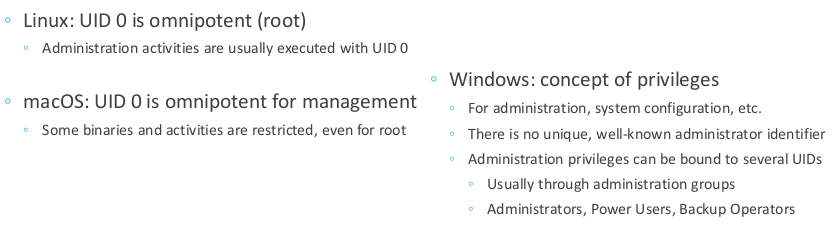
\includegraphics[scale=0.4]{29}
\end{center}

\subsection{Identificadores de Grupo (GID)}

\begin{flushleft}
  \textbf{OS também têm group identifiers}. Um grupo é composto por 0 ou mais
  users e pode ser composto por outros grupos. Group ID: inteiro (Linux,
  Android, macOS), UUID (Windows).

  \vspace{2mm}

  \textbf{Um user pode pertener a vários grupos}. Os direitos de um user são
  o direito do seu UID e dos seus GID's.

  \vspace{2mm}

  \textbf{Em Linux, as atividades executam sempre por baixo do scope de um
  conjunto de grupos}. 1 grupo primário (ownership dos ficheiros criados),
  múltiplos secundários (condicionam o acesso aos recursos).
\end{flushleft}

\subsection{Processos}

\begin{flushleft}
  \textbf{Um processo define o contexto da atividade}, para tomar decisões
  relacionadas com segurança ou outros propósitos (e.g scheduling).

  \vspace{2mm}

  \textbf{Contexto relacionado à segurança}. Identidade efetiva (eUID e eGID),
  fundamental para controlo de acesso, pode ser o mesmo que a identificação
  do user que lança o processo. Os recursos usados são ficheiros abertos,
  areas reservadas de memória virtual, \dots
\end{flushleft}

\subsection{Memória Virtual}

\begin{flushleft}
  \textbf{O espaço de endereçamento onde a atividade acontece}, tem o tamanho
  máximo definido pela arquitetura do sistema (32 bits $\rightarrow$ $2^{32}$,
  64 bits $\rightarrow$ $2^{64}$). Gere em pequenos blocos de memória, páginas
  (4KiB).

  \vspace{2mm}

  \textbf{Memória virtual pode ser escassa}, uma vez que, apenas as páginas
  usadas devem ser alocadas.

  \pagebreak

  \textbf{Memória virtual é mapeada a RAM quando usada}. A escolha de como
  gerir estes espaços é muito importante (evitar fragmentação, \dots).
\end{flushleft}

\begin{center}
  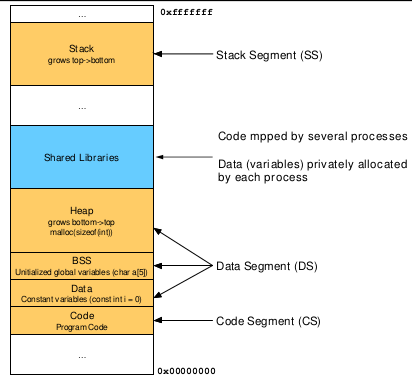
\includegraphics[scale=0.4]{30}
\end{center}

\subsection{Sistema de Ficheiros}

\begin{center}
  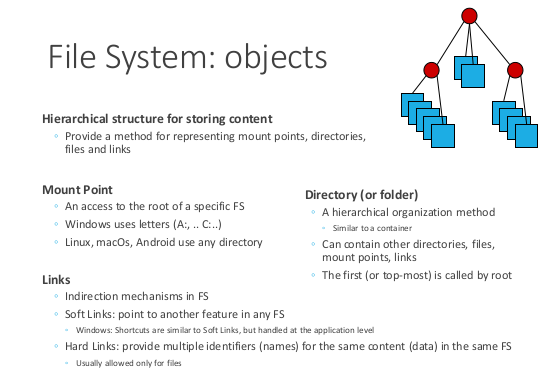
\includegraphics[scale=0.4]{31}
  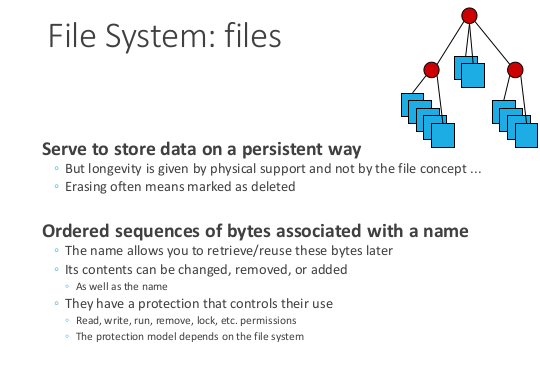
\includegraphics[scale=0.4]{32}
\end{center}

\pagebreak

\subsubsection{Sistema de Ficheiros: Mecânismos de Segurança}

\begin{flushleft}
  \textbf{Mecânismos de proteção obrigatórios}, para o owner,
  users e grupos são permitidos. Permissões são Read, Write e Run.

  \vspace{2mm}

  \textbf{Mecânismos de proteção discricionários}, regras específicas
  para users.

  \vspace{2mm}

  \textbf{Mecânismos adicionais}, como implicit compression,
  signature, encryption, \dots
\end{flushleft}

\subsection{Canais de Comunicação}

\begin{flushleft}
  \textbf{Permitem a troca de dados entre atividades distintas mas cooperativas}.

  \vspace{2mm}

  \textbf{Esta presente em qualquer sistema}, todas as aplicações usam estes
  mecânismos.

  \vspace{2mm}

  \textbf{Processos no mesmo SO/máquina}, através de pipes, UNIX sockets,
  streams, \dots Comunicação entre processos e kernel, através de system calls, sockets.

  \vspace{2mm}

  \textbf{Processos em máquinas diferentes}, TCP/IP e UDP/IP sockets.
\end{flushleft}

\subsection{Controlo de Acesso}

\begin{flushleft}
  \textbf{O kernel do OS é um monitor de controlo de acesso}, controla
  todas as interações com o hardware. As alicações nunca usam recursos
  diretamente e também controla todas as interações entre computational model
  entities.

  \vspace{2mm}

  \textbf{Sujeitos} são tipicamente processos locais, mas também mensagens de outras
  máquinas.
\end{flushleft}

\begin{center}
  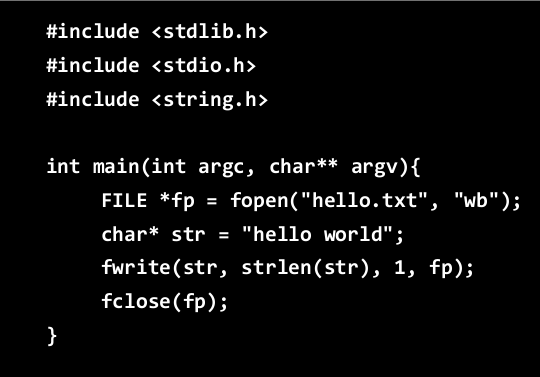
\includegraphics[scale=0.3]{33}
  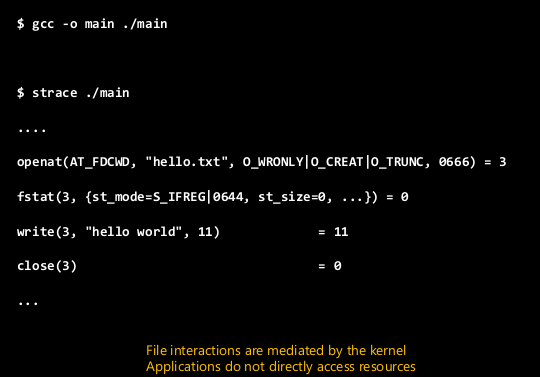
\includegraphics[scale=0.3]{34}
\end{center}

\subsection{Controlo de Acesso Obrigatório}

\begin{flushleft}
  \textbf{Há muitos casos de controlo de acesso obrigatório no OS},
  parte dá lógica do modelo computacional, não são moldáveis por users ou
  administradores.

  \vspace{2mm}

  \textbf{Exemplos em Linux:} A root pode fazer tudo, os sinais para processos
  são enviados apenas pela root ou pleo owner.

  \textbf{Exemplos em macOS:} A root faz quase tudo, mas não pode alterar binários
  e dirétorias da Apple.
\end{flushleft}

\pagebreak

\subsection{Controlo de Acesso Discricionário}

\begin{flushleft}
  \textbf{Users podem criar um conjunto de regras de controlo de acesso},
  podem ser definidas apenas pelo owner/user.

  \vspace{2mm}

  \textbf{Exemplo:}

  \begin{itemize}
    \item \textbf{Discretionary Access Control Lists (ACL)}, listas expressivas que
    limitam o acesso a recursos em Linux;
    \item \textbf{Linux Apparmor}, guarda settings em /etc/apparmor.d com limites de
    aplicações. As regras aplicam-se automaticamente aos processos, independentemente
    do user;
    \item \textbf{macOS sandboxd}, aplicações são lançadas em contextos isolados (sandbox),
    esta sandbox contém informação sobre o que entra/sai;
  \end{itemize}
\end{flushleft}

\end{document}